% example tikz figure

\documentclass{standalone}
\usepackage{amsmath}
\usepackage{amsfonts}
\usepackage{tikz}
\usetikzlibrary{arrows,shapes,positioning,shadows,trees}


\begin{document}
\begin{tikzpicture}
    % mark center with x mark
    \draw[-] (0,0) -- (0,0) node[anchor=center] {$\times$};

    \draw [->] plot [smooth, tension=1, circle] coordinates {(1.75,0) (1,1.5) (0,1) (-2,0.5) (0,-1) (1.5,-0.8) (1.75,0)};

    % label as \gamma
    \node[above right] at (1.75,0) {$\gamma$};
\end{tikzpicture}
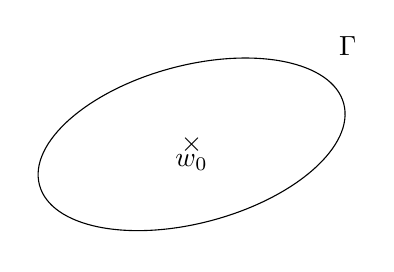
\begin{tikzpicture}
    % mark center with x mark
    \draw[-] (0,0) -- (0,0) node[anchor=center] {$\times$};
    \node[below] at (0,0) {$w_0$};

    \draw (0,0) [rotate=15] ellipse (2cm and 1cm);

    % label as \gamma
    \node[above right] at (1.75,1) {$\Gamma$};
\end{tikzpicture}

\begin{tikzpicture}
    \node (a) at (0,0) {
        \begin{tikzpicture}
            \filldraw[fill=gray!30, draw=black] (0,1.732) circle (2);
            \filldraw[fill=white, draw=black] (0,0) circle (1);
            \draw[->] (-2,0) -- (2,0);
            \draw[->] (0,-2) -- (0,4);
            % draw |z| = 1 circle
            \draw (0,0) circle (1);
            % draw |z - sqrt(3)i| = 2 circle
            \draw (0,1.732) circle (2);

            % label \sqrt(3) i, -1 with filled dot
            \node[fill,circle,inner sep=1pt,label=above right:$\sqrt{3}i$] at (0,1.732) {};
            \node[fill,circle,inner sep=1pt,label=below left:$-1$] at (-1,0) {};
            % fill O, 1, no label
            \node[fill,circle,inner sep=1pt] at (0,0) {};
            \node[fill,circle,inner sep=1pt] at (1,0) {};
        \end{tikzpicture}
    };

    \node(b) at (6,0) {
        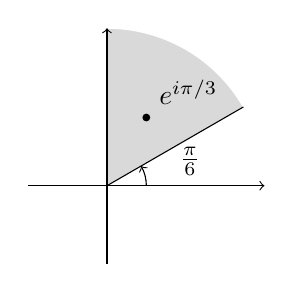
\begin{tikzpicture}
            % fill \theta > pi/6, \theta < pi/2
            \filldraw[fill=gray!30, draw=white!0] (0,0) -- (1.732,1) arc (30:90:2) -- (0,0);

            \draw[->] (-1,0) -- (2,0);
            \draw[->] (0,-1) -- (0,2);

            \draw[-] (0,0) -- (1.732, 1);
            % label angle with arc, radius 0.5
            \draw[->] (0.5,0) arc (0:30:0.5);
            % label pi/6
            \node[above right] at (0.8,0) {$\frac{\pi}{6}$};

            % mark exp(i pi/3) with filled dot
            \node[fill,circle,inner sep=1pt,label=above right:$e^{i\pi/3}$] at (1 / 2,1.732 / 2) {};
        \end{tikzpicture}
    };

    \node (c) at (12,0) {
        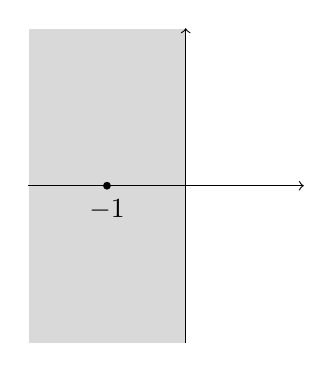
\begin{tikzpicture}
            % fill Re z < 0 with rectangle
            \filldraw[fill=gray!30, draw=white!0] (-2,2) -- (-2,-2) -- (0,-2) -- (0,2) -- (-2,2);
            \draw[->] (-2,0) -- (1.5,0);
            \draw[->] (0,-2) -- (0,2);

            % mark (-1,0)
            \node[fill,circle,inner sep=1pt,label=below:$-1$] at (-1,0) {};
        \end{tikzpicture}
    };

    \node (d) at (18,0) {
        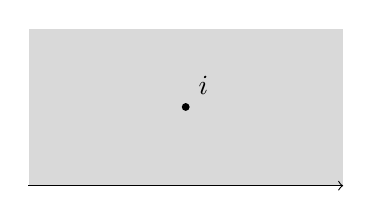
\begin{tikzpicture}
            % rotate c -90 degrees
            \filldraw[fill=gray!30, draw=white!0] (-2,2) -- (-2,0) -- (2,0) -- (2,2) -- (-2,2);
            \draw[->] (-2,0) -- (2,0);

            % mark i
            \node[fill,circle,inner sep=1pt,label=above right:$i$] at (0,1) {};
        \end{tikzpicture}
    };

    \node (e) at (24,0) {
        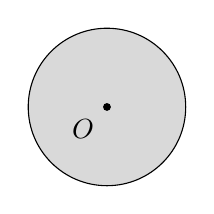
\begin{tikzpicture}
            % circle |z| = 1, fill
            \filldraw[fill=gray!30] (0,0) circle (1);

            % label O
            \node[fill,circle,inner sep=1pt,label=below left:$O$] at (0,0) {};
        \end{tikzpicture}
    };

    % from a to b, f(z) = \dfrac{z+1}{z-1}
    \draw[->,thick] (a) -- (b) node[midway,above] {$f(z) = \dfrac{z+1}{z-1}$};
    % from b to c, f(z) = z^3
    \draw[->,thick] (b) -- (c) node[midway,above] {$f(z) = z^3$};
    % from c to d, f(z) = -iz
    \draw[->,thick] (c) -- (d) node[midway,above] {$f(z) = -iz$};
    % from d to e, f(z) = exp[i\theta]\cdot\dfrac{z-i}{z+i}
    \draw[->,thick] (d) -- (e) node[midway,above] {$f(z) = e^{i\theta}\cdot\dfrac{z-i}{z+i}$};
\end{tikzpicture}

\end{document}